This chapter provides examples of memory persistency models and data structures using the memory persistency framework defined in the previous chapter.
I first introduce a concurrent, persistent queue, outlining several design choices and reasoning about persist performance.
I then define specific memory persistency models under sequential consistency (SC), demonstrating their use with the persistent queue.
The final chapter of this dissertation evaluates these persistency models using the persistent queue.

\section{Persistent Queue}
\label{sec:PersistencyModels:Queue}

To understand and evaluate persistency models I first introduce a motivating benchmark: a thread-safe persistent queue.
Several workloads require high-performance persistent queues, such as write ahead logs (WAL) in databases and journaled file systems.
Previous work investigated the design of an NVRAM log assuming byte-addressable NVRAM with a persist barrier \cite{FangHsiao11}.
I extend this work, outlining three queue designs with several persistency models.

Fundamentally, a persistent queue inserts and removes entries while maintaining their order.
The queue must recover after failure, preserving proper entry values and order.

My goals in designing a persistent queue are to (1) maximize the instruction execution rate, including multi-thread throughput, (2) improve the persist concurrency of insert operations through greater thread concurrency, and (3) further improve persist concurrency using relaxed persistency.
All designs are concurrent (thread-safe) but allow varying degrees of persist concurrency.
Additionally, the three designs are fashioned as circular buffers, containing a data segment and head and tail pointers.
Psuedo-code for the three designs is shown in Figure~\ref{Alg::Queue}.
I outline their execution, recovery, and the minimal necessary persist dependences.

\begin{figure}

%\begin{algorithm}
  \caption{\textbf{Psuedo-code for insert operations.}  I include the annotations required by relaxed persistency models, discussed in Section~\ref{sec:PersistencyModels:Models}.  $PersistBarrier$ applies to epoch persistency and strand persistency, $NewStrand$ applies only to strand persistency.}
  \label{Alg::Queue}
  \begin{algorithmic}[1]
  \Require $head$ is a persistent pointer, $data$ a persistent array.
  \State $sl \gets$ \Call{sizeof}{length}
  \Function{InsertCWL}{$length$, $entry$}
    \State \Call{lock}{$queueLock$}
    \State \Call{NewStrand}{}
    \State \Call{copy}{$data[head]$, ($length$, $entry$), $length+sl$}
    \State \Call{PersistBarrier}{}
    \State $head \gets head+length+sl$
    \State \Call{unlock}{$queueLock$}
  \EndFunction
  \State
  \Function{Insert2LC}{$length$, $entry$}
    \State \Call{lock}{$reserveLock$}
    \State $start \gets headV;$ $headV \gets headV+length+sl$
    \State $node \gets insertList$.\Call{append}{$headV$}
    \State \Call{unlock}{$reserveLock$}
    \State \Call{NewStrand}{}
    \State \Call{copy}{$data[head]$, ($length$, $entry$), $length+sl$}
    \State \Call{lock}{$updateLock$}
    \State ($oldest$, $newHead$) $\gets insertList$.\Call{remove}{$node$}
    \State \Call{unlock}{$updateLock$}
    \If{$oldest$}
      \State \Call{PersistBarrier}{}
      \State $head \gets newHead$
    \EndIf
    \State $unlock(reserveLock)$
  \EndFunction
  \State
  \Function{InsertQH}{$length$, $entry$}
    \State \Call{lock}{$queueLock$}
    \State \Call{NewStrand}{}
    \State $start \gets head$; $endPos \gets start+length+sl$ %\Comment{marks $endBit$}
    \State $data[start] \gets length$; $data[endPos] \gets 0$
    \State \Call{PersistBarrier}{}
    \State $head \gets head+length+sl+1$
    \State \Call{unlock}{$queueLock$}
    \State \Call{copy}{$data[start+sl]$, $entry$, $length$}
    \State \Call{PersistBarrier}{}
    \State $data[endPos] \gets 1$
  \EndFunction
  \end{algorithmic}
%\end{algorithm}

\end{figure}


The first design, \emph{Copy While Locked} (CWL), serializes insert operations with a lock, first persisting each entry's length and data to the queue's data segment, then persisting the new head pointer.
As a result, persists from subsequent insert operations, even if they occur on separate threads, are ordered by lock accesses.
If the systems fails before the persist to the head pointer in line 6, the entry is ignored and the insert has failed.

I improve persist concurrency in the second design, \emph{Two-Lock Concurrent} (2LC), by using two different locks to reserve data segment space and persist to the head pointer, respectively.
Neither lock is held while entry data persists to the data segment, allowing concurrent persists from different threads.
Additionally, a volatile \emph{insert list} is maintained to detect when insert operations complete out of order and prevent holes in the queue.
The double-checked locking pattern prevents data races while updating the insert queue.
\emph{Two-Lock Concurrent} employs the same recovery as \emph{Copy While Locked}---an entry is not valid and recoverable until the head pointer encompasses the associated portion of the data segment.

\begin{figure}
  \centering
  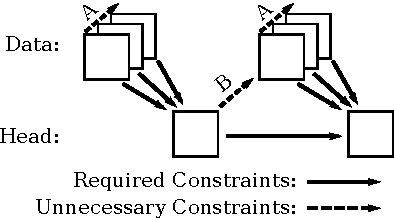
\includegraphics[width=.55\linewidth]{PersistencyModels/CWL_2LC_dependences.pdf}
  \caption{\textbf{Queue Persist Dependences.} Persist ordering dependences for \emph{Copy While Locked} and \emph{Two-Lock Concurrent}.  Constraints necessary for proper recovery shown as solid arrows; unnecessary constraints incurred by strict persistence appear as dashed arrows and are labelled as A (removed with epoch persistency) and B (further removed by strand persistency).}
  \label{fig::CWL_dependences}
\end{figure}


Both queue designs use the persistency model to prevent persists to the head pointer from occurring before persists to the data segment.
Figure~\ref{Alg::Queue} includes barriers for two different persistency models (described later in Section~\ref{sec:PersistencyModels:Models}).
Additionally, persist dependences (and unnecessary constraints introduced by strict persistency models) are shown in Figure~\ref{fig::CWL_dependences}.
Recovery requires that persists to the head pointer are ordered after persists to the data segment from the same insert operation and persists to the head pointer occur in insert-order to prevent holes in the queue (persists to the head pointer may coalesce so long as no ordering constraint is violated).
All other persists within the same insert operation and between operations may occur concurrently without compromising recovery correctness.

While not necessary for correct recovery, these persist dependences are difficult to describe minimally; ordering mechanisms often introduce unnecessary persist constraints (dashed lines in the Figure).
Persistency models that enforce program order of persists in each thread must serialize persists for the data of each entry to the data segment (when the entire entry cannot be persisted atomically), shown as ``A" in the Figure.
Additionally, persists to the data segment may be ordered after a previous insert's persist to the head pointer, denoted as ``B" in the Figure.

The previous designs trade off concurrency and complexity.
\emph{Copy While Locked}, while simple, serializes persists between insert operations.
On the other hand, \emph{Two-Lock Concurrent} allows greater concurrency, but requires two locks be acquired per insert and a volatile \emph{insert list} be maintained.
I consider a third design, \emph{Queue Holes}, that provides both improved persist concurrency and a high execution rate (first introduced in \cite{FangHsiao11}).

\begin{figure}
  \centering
  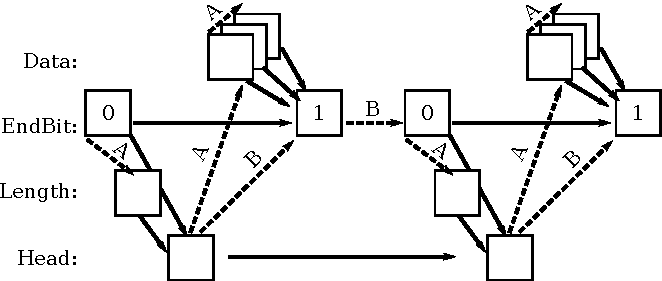
\includegraphics[width=\linewidth]{PersistencyModels/holes_dependences.pdf}
  \caption{\textbf{\emph{Queue Holes} Dependences.} The head pointer may not persist before \emph{endBit} and length; final \emph{endBit} may not persist until the entry persists to the data segment.  Strict persistency introduces several unnecessary constraints.}
  \label{fig::holes_dependences}
\end{figure}


\emph{Queue Holes} prepends each queue entry with its length and appends the entry with an endBit.
A single lock is held while reserving queue space and updating the head pointer, but is released prior to persisting the entry into the data segment.
An entry is recovered after failure if the entry is located within the region indicated by the head pointer (as in CWL and 2LC) and the entry's endBit is set.
The minimal set of persist dependences necessary for correct recovery are shown in Figure~\ref{fig::holes_dependences}.
The length and cleared endBit persist before the head pointer; the data segment persists before setting the endBit; and persists to the same address occur in the order observed by cache coherence (endBits and the head pointer).
An inserted entry is recoverable only after the persist at line 37 completes, even though the head pointer is persisted earlier at line 33.

As with the other queue designs many unnecessary persist constraints may be introduced by strict persistency models, shown as dashed lines in Figure~\ref{fig::holes_dependences}.
Many constraints are introduced by persistency models that enforce the program order of persists, labeled ``A."
Additional constraints may be introduced between persists within an insert operation or across insert operations, labeled ``B."

\section{Memory Persistency Models}
\label{sec:PersistencyModels:Models}

Section~\ref{sec:Persistency:Persistency} outlined potential classes of persistency models.
I now introduce several specific persistency models to be evaluated in the next chapter.
All models assume SC as the underlying memory consistency model, and successively relax persistency to introduce specific optimizations.
For each model I discuss its motivation, give a definition, describe necessary annotations for and performance of the persistent queues, and offer possible implementations.

\subsection{Strict Persistency}
\label{section:PersistencyModels:Strict}

\textbf{Motivation.}
The first persistency model is Strict Persistency, as discussed in Section~\ref{sec:Persistency:Persistency}.
Strict persistency simplifies reasoning about persist ordering by coupling persist dependences to the memory consistency model.
No additional persist barriers are required, easing the burden on the programmer.
While strict persistency provides an intuitive first model, under SC, it imposes persist ordering constraints that unnecessarily limit persist concurrency for many data structures, and requires programmers to resort to multi-threading to obtain concurrency.

\textbf{Definition.}
Under strict persistency, persist order observes all happens-before relations implied by execution's dynamic order of memory operations as viewed by the recovery observer.
Thus, all persists are ordered with respect to the program order of the issuing thread.
Note that, like store operations, persists from different threads that are unordered by happens-before (i.e., the recovery observer cannot distinguish which is first) are concurrent.

\textbf{Persist Performance.}
Strict persistency under SC introduces many unnecessary persist dependences.
Consequently, strict persistency must rely entirely on thread concurrency to enable concurrent persists.
Figures~\ref{fig::CWL_dependences} and~\ref{fig::holes_dependences} illustrate these unnecessary dependences and their causes.
Lacking mechanisms to relax persist ordering, strict persistency under SC introduces all the shown dependences (dashed lines).

These dependences are introduced because persists occur in program order under SC.
This persistency model lacks the ability to declare two persists from the same thread to be concurrent.
However, persist concurrency may be created by using multiple threads to concurrently insert into the queue.
\emph{Two-Lock Concurrent} and \emph{Queue Holes} each allow concurrent inserts, and thus persists from different threads into the data segment are concurrent---The dashed line labeled ``B" in Figure~\ref{fig::CWL_dependences} no longer implies a constraint.

\textbf{Implementation.}
A straight-forward implementation of strict persistency stalls issue of subsequent memory accesses until a store and its corresponding persist both complete.
Conventional speculation mechanisms may allow loads to speculatively reorder with respect to persistent stores \cite{Gharachorloo91}.
Buffered strict persistency can be implemented by serializing persists to a single, totally ordered queue in front of persistent memory (e.g., in a bus-based multiprocessor, persists can be queued after they are serialized by the bus).
Delays still occur when buffers fill, to drain the queue at persist sync instructions, or under contention to the persist queue.

More advanced implementations might consider distributed queues (i.e., one queue per thread/core) or extensions to the existing cache system.
Mechanisms must be introduced to ensure that persists of each thread occur in program order and that persists are ordered by conflicting accesses from different threads, but persists from several threads may occur concurrently (they are not serialized) while persists buffer and execution proceeds ahead of persistent state.
Under the definition of SC such implementations must detect load-before-store races between threads, ordering persists prior to the load (on the first thread) before persists after the store (on the second thread).
A single store may introduce persist ordering constraints with many threads, each having loaded data from the store's address.
It is unclear how to design a system that satisfies these constraints without frequent delays.

While insufficient for SC, TSO might be implemented by recording a ``persist counter" and thread in each cache line.
Each time a thread persists it increments its persist counter, and each store (both volatile stores and persists) writes the thread and persist counter into the cache line.
Persists drain in program order by maintaining a persist queue per thread/core.
Persist order between threads is enforced at each load and store by observing the previously recorded thread and counter in the operation's cache line---all subsequent stores from the executing thread must occur after the last persist to the cache line.
These inter-thread persist constraints may be recorded in threads' queues or by delaying immediately until the other thread's queue drains.
Such a system resembles BPFS (discussed next in Section~\ref{section:PersistencyModels:PersistEpochs} and later in Section~\ref{sec:PersistencyModels:RelatedWork}) where each persist occurs in its own epoch \cite{ConditNightingale09}.

Strict persistency under SC may also be implemented using in-hardware NVRAM logs or copy-on-write and indirection to give the appearance of SC while persists occur concurrently.
Hardware must ensure both that persists do not occur out of program order for any thread and that conflicting accesses properly enforce persist order across threads.
An intriguing possibility would be to leverage existing hardware transactional memories (HTM), partitioning program execution into transactions that enforce atomicity, isolation, and durability---resembling BulkSC with durable transactions \cite{CezeTuck07}.
Transactions must be long enough to minimize transaction overhead (including persist barriers for each durable transaction) and improve persist concurrency (by placing many persists in the same transaction), but short enough to bound resources necessary for atomic transactions (such as a log) and to minimize forward progress lost when a transaction aborts.
%Additionally, transactions may buffer persists so long as transactions become visible to recovery in their proper order.
%I leave it to future work to investigate how to coalesce persists between durable transactions.

\subsection{Epoch Persistency}
\label{section:PersistencyModels:PersistEpochs}

\textbf{Motivation.}
Strict persistency under SC introduces many persist dependences unnecessary for correct recovery.
The most common unnecessary persist dependence occurs due to the program-order constraint of SC.
Programs frequently persist to large, contiguous regions of memory that logically represents a single object, but which cannot occur atomically (due to their size).
Under strict persistency, the persists serialize.
I remove the program-order-implied persist order constraint with \emph{epoch persistency}, allowing consecutive persists from the same thread to reorder and persist in parallel.
Doing so, however, requires annotation by the programmer in the form of persist barriers to divide execution into epochs when ordering is required by the recovery algorithm.
Epoch persistency additionally allows persists to addresses protected by a lock to reorder with respect to the lock operations (e.g., avoid delaying the lock release while the persist completes); my queue implementations leverage this optimization opportunity.

\textbf{Definition.}
Epoch persistency defines a new \emph{persistent memory order} in addition to execution's existing memory order (referred to as the \emph{volatile memory order}).
Persistent memory order contains a subset of constraints from the volatile memory order.
Any pair of persists ordered in the persistent memory order may not be observed out of that order with respect to the recovery observer.

Volatile memory order satisfies SC.
Each thread's execution is additionally separated into \emph{persist epochs} by persist barrier instructions.
Epoch persistency provides several rules to inherit memory order constraints from the volatile memory order: (1) any two memory accesses on the same thread separated by a persist barrier assume the order observed from volatile memory order (program order), (2) any two memory accesses (from the same or different threads) that conflict (they are to the same or overlapping addresses and at least one is a store/persist) assume the order observed from volatile memory order (typically enforced via cache coherence), and (3) eight-byte persists are atomic with respect to the recovery observer and failure.
This last rule is somewhat relaxed in my evaluation, requiring only that eight-byte and \emph{aligned} persists be atomic.

Persist barriers enforce that no persist after the barrier may occur before any persist before the barrier.
Persists within each epoch (not separated by a barrier) are concurrent and may reorder or occur in parallel.
Additional complexity arises in reasoning about persist ordering across threads. 
I define a \emph{persist epoch race} as persist epochs from two or more threads that include memory accesses (to volatile or persistent memory) that race, including synchronization races, and at least two of the epochs include persist operations. 
In the presence of a persist epoch race, rules (1) and (2) order accesses prior to the epoch of the earlier access in the race before accesses following the epoch of the later access in the race.
Additionally, conflicting accesses are themselves ordered according to the volatile memory order.
Consequently, two persists to the same address are always ordered even if they occur in racing epochs.

\textbf{Discussion.}
Epoch persistency provides an intuitive mechanism to guarantee proper recovery as it is impossible at recovery to observe a persist from after a barrier while failing to observe a persist from before the same barrier.
However, many persists (those within the same epoch) are free to occur in parallel, improving persist concurrency.

As noted in the definition, reasoning about persist order across threads can be challenging.
Synchronization operations within persist epochs impose ordering across the store and load operations (due to SC memory ordering), but do not order corresponding persist operations.
Hence, persist operations correctly synchronized under SC by volatile locks may nevertheless result in astonishing persist ordering.
A simple (yet conservative) way to avoid persist epoch races is to place persist barriers before and after all lock acquires and releases, and to only place locks in the volatile address space.
The persist behavior of strict persistency can be achieved by preceding and following all persists with a persist barrier.

Persist epoch races may be intentionally introduced to increase persist concurrency; I discuss such an optimization below.
Enforcing persist order between threads with volatile locks requires that the persists be synchronized outside of the epochs in which the persists occur.
However, synchronization through persistent memory is possible.
Since persists to the same address must follow the order observed by cache coherence, even if they occur in epochs that race, the outcome of persist synchronization is well defined.
Hence, atomic read-modify-write operations to persistent memory addresses provide the expected behavior.

\textbf{Persist ordering example.}
\begin{figure}
  \centering
  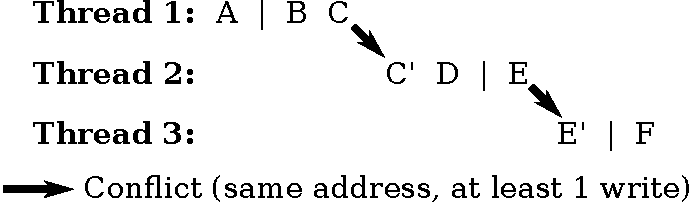
\includegraphics[width=.55\linewidth]{PersistencyModels/propagation.pdf}
  \caption{\textbf{Epoch persistency persist order.} Persistent memory order is enforced through persist barriers (shown as `` $\vert$ ") and access conflicts.  Access A is ordered by transitivity before access F.  If these accesses are persists they may not be reordered with respect to the recovery observer.  This order is enforced even if accesses are to the volatile address space.  Access B is concurrent with all shown accesses from threads 2 and 3, while access D is concurrent with accesses from thread 1.}
  \label{fig::EpochPersistencyPropagation}
\end{figure}

Figure~\ref{fig::EpochPersistencyPropagation} demonstrates a sample memory execution and the resulting persistent memory order.
Capital letters denote memory accesses (loads, stores, and persists), accesses labeled by the same letter are to the same address.
`` $\vert$ " implies a persist barrier.
Arrows show access conflicts and the order that the conflict is observed in volatile memory order.

According to rule (1) of epoch persistency all accesses on the same thread are ordered if separated by a persist barrier (A before B and C; C' and D before E; and E' before F).
By rule (2) all conflicts are ordered according to volatile memory order (C before C'; E before E').
Transitivity of these rules additionally orders accesses (A before C', E, E', and F; C before E, E', and F; C' and D before E' and F; and E before F).
Notably, B is unordered with all shown accesses by threads 2 and 3, and D is unordered with accesses by thread 1 (such accesses are concurrent).
Any accesses that are persists may not be observed out of this order by the recovery observer (e.g., a persist to F may not be observed while a persist to A is not).

This order is enforced on conflicts (between C and C'; E and E') to both volatile and persistent address spaces and as long as one of the accesses is a store or persist.
This includes the case where the first access is a load and the second a store/persist.
Providing an implementation to enforce this constraint remains a challenge, as persists must complete before a subsequent load executes or all load-store conflicts must be detected and enforced at some later time.

The resulting persist order resembles RMO \cite{SPARCv9} with (at least) one important difference: memory order constraints introduced due to control and register data dependencies do not impose a persistent memory order constraint in epoch persistency.
For example, consider that access C is a persist, C' a load, and D a persist whose value depends on C'.
According to RMO such a register dependence initiated by a load introduces a (volatile) memory order constraint.
Strict persistency under RMO would now allow persist D to be observed without also observing persist C.
Epoch persistency, on the other hand, allows such behavior, violating RMO.
In general persistent memory order need not order accesses that contain a register dependence, but this may produce unintuitive or unintended behavior.

\textbf{BPFS.}
My definition of epoch persistency is inspired by the programming model and hardware extensions for caching persistent memory proposed for the Byte-addressable Persistent File System (BPFS) \cite{ConditNightingale09}.
However, I introduce several subtle differences that I believe make epoch persistency a more intuitive model.
My definition considers all memory accesses when determining persist ordering among threads, whereas the BPFS memory system orders persists only when conflicts occur to the persistent address space.
While the BPFS file system implementation avoids persist epoch races, it is not clear that the burden falls to the programmer to avoid such accesses or what persist behavior results when such races occur (I believe the BPFS authors' intent was to prohibit programs containing such races---the cache implementation deadlocks under persist epoch races containing circular persist dependences).  
Furthermore, BPFS detects conflicts to the persistent address space by recording the last thread and epoch to persist to each cache line; the next thread to access that line will detect the conflict.
Such an implementation, however, cannot detect conflicts where the first access is a load and the second a store.
While occasionally unintuitive, such behavior rarely results in unintended behavior and greatly simplifies the memory system.
Existing memory consistency models similarly order accesses, including TSO \cite{SPARCv9}).

\textbf{Persist Performance.}
Epoch persistency removes all unnecessary persist dependences that result from strict persistency's program order constraint.
All versions of the persistent queue benefit from allowing persist entries to persist to the data segment concurrently.
Additionally, \emph{Queue Holes} allows entry length and \emph{endBit} to persist concurrently (although both are ordered with respect to the subsequent persist of the head pointer).
Finally, many persist constraints between threads are removed by intentionally allowing persist epoch races.
Lock operations occur in the same epoch as the first persists of the insert operation, while unlock operations occur in the same epoch as the last persists; persists from the last epoch of an insert and the first epoch of the subsequent insert are concurrent.
As a result, persists protected by a lock now occur concurrently.
\emph{Copy While Locked} and \emph{Queue Holes} retain recovery correctness by still ordering all persists to the head marker (persists occur according to cache coherence order).

Figure~\ref{Alg::Queue} demonstrates how to use epoch persistency's barriers (shown in the code as $PersistBarrier$) within each queue design.
The constraints in Figures~\ref{fig::CWL_dependences} and~\ref{fig::holes_dependences} annotated with ``A" are removed under epoch persistency relative to strict persistency.

\textbf{Implementation.}
BPFS \cite{ConditNightingale09} outlines cache extensions that provide a persistency model similar to persist epochs, assuming the TSO consistency model.
Modifications must be made to detect load-before-store conflicts (and thus enforce SC rather than TSO ordering) and track conflicts to volatile memory addresses as well as persistent memory addresses; detecting load-before-store conflicts and enforcing persist order without frequent delays remains an open problem.
Instead of delaying execution to enforce persist ordering among threads, optimized implementations avoid stalling execution by buffering persists while recording and subsequently enforcing dependences among them, allowing persists to occur asynchronously despite access conflicts.

More advanced techniques might rely on hardware NVRAM logging and hardware transactional memory, partitioning program execution into transactions as discussed above for strict persistency.
Under epoch persistency any transaction that contains only a single epoch need not persist atomically, and therefore logging is unnecessary (persist order must still be enforced between transactions).
Persist barriers may be used as hints to establish transaction boundaries and minimize durable transaction logging.

\subsection{Strand Persistency}
\label{section:PersistencyModels:PersistStrands}

\textbf{Motivation.}
Epoch persistency relaxes persist dependences within and across threads.
However, only consecutive persists within a thread may be labeled as concurrent.
Likewise, persists from different threads are only concurrent if their epochs race or if they are not synchronized.
Many persists within and across threads may still correctly be made concurrent even if they do not fit these patterns.
I introduce \emph{strand persistency}, a new model to minimally annotate persist dependences.

\textbf{Definition.}
A strand is an interval of memory execution from a single thread.
Strands are separated via \emph{strand barriers}; each strand barrier begins a new strand.
The strand barrier clears all previously observed persist dependences from the executing thread.
Within each strand new and observed persists are ordered using persist barriers according to the epoch persistency model.
Rule (1) of epoch persistency may be modified to read: any two memory accesses on the same \emph{strand} separated by a persist barrier assume the order observed from volatile memory order (accesses from different strands never assume a program order constraint, and will only be ordered through conflicts or ordering constraints with accesses in the same strand).
Rules (2) and (3) of epoch persistency apply without modification.

\textbf{Discussion.}
There are no implicit persist ordering constraints across strands for persists to different addresses on the same thread of execution.
Ordering constraints arise only for persists to the same address as implied by cache coherence.
Hence, persists on a new strand may occur as early as possible and overlap with all preceding persists.
Strand persistency allows programmers to indicate that logical tasks on the same thread are independent from the perspective of persistency.
To enforce necessary ordering, a persist strand begins by reading any memory locations after which new persists must be ordered.
These reads introduce an ordering dependency due to cache coherence, which can then be enforced with a subsequent persist barrier.
This programming interface allows ordering constraints to be specified at the granularity of individual addresses; the minimal set of persist dependences is achieved by placing each persist in its own strand, loading all addresses the persist must depend on, inserting a persist barrier, and then executing the persist.

The performance of epoch persistency is achieved by using a single persist strand on each thread (strand persistency is equivalent to epoch persistency under such conditions).
While I enforce persist order within strands according to epoch persistency, other persistency models may be used (e.g., strict persistency/SC orders persists within strands but new strands clear previously observed dependences).

While intended for persistency, strand persistency additionally functions as a consistency model (\emph{strand consistency}).
Strand consistency requires full memory barriers in lieu of persist barriers; loads and stores may not reorder across memory barriers.
Additionally, the execution of loads and stores may not reorder across strand barriers for the purpose of observing memory dependences between strands on the same thread, but loads and stores from different strands that do not interact may reorder with respect to other processors and threads.
Dependences propagate through memory execution and cache coherence, with strands from the same thread being concurrent if they do not share conflicts through memory (i.e., the visibility of loads and stores from different strands may reorder).
Recent trends suggest that such a relaxed consistency model is unnecessary for typical memory architectures as memory systems have tended towards stricter models with improved performance.

\textbf{Persist Performance.}
The persistent queue implementations place each insert task in a separate persist strand.
The result is that all unnecessary persist constraints are removed, including constraints between inserts from the same thread.
Figure~\ref{Alg::Queue} includes the necessary strand persistency annotations ($NewStrand$ and $PersistBarrier$).
All unnecessary constraints from Figures~\ref{fig::CWL_dependences} and~\ref{fig::holes_dependences} are removed; those removed in moving from epoch persistency to strand persistency are labeled ``B."
The required persist dependences (and only those required for correct recovery) remain, maximizing persist concurrency.

\textbf{Implementation.}
Strand persistency builds on the hardware requirements to track persist dependencies as in epoch persistency, but further requires mechanisms to separate tracking of dependencies for different strands.
In addition to tracking the last thread to access each persistent location, the strand within the thread must also be tracked.
Unordered persists on different strands can traverse separate queues (e.g., on separate virtual channels) throughout the persistent memory system.
Strand persistency gives enormous implementation latitude and designing efficient hardware to track and observe only the minimal ordering requirements remains an open research challenge.
In this work, I focus on demonstrating the potential performance that the model allows.

\section{Related Work}
\label{sec:PersistencyModels:RelatedWork}

Durable storage has long been used to recover data after failures.
All systems that use durable storage must specify and honor dependencies between the operations that update that storage.
For example, file systems must constrain the order of disk operations to metadata to preserve a consistent file system image~\cite{Ganger00,Chidambaram13}, and databases must obey the order of durable storage updates specified in write-ahead logging~\cite{MohanHaderle92}.

Specifying and honoring these dependencies becomes harder when the interface to durable storage are loads and stores to a persistent address space.
Store instructions to an address space are more frequent and fine grained than update operations when using a block-based interface to durable storage (such as a file system).
In addition, CPU caches interpose on store instructions, which leads to the interaction of persistency and cache consistency discussed in this dissertation.

Recent developments in nonvolatile memory technologies have spurred research on how to use these new technologies.
Some research projects keep the traditional block-based interface to durable storage and devise ways to accelerate this interface~\cite{CaulfieldDe10}.
Other projects provide a memory-based interface to durable storage~\cite{CoburnCaulfield11}.
My approach follows the path of providing a memory-based interface to durable storage, arguing that the high speed and fine-grained access of new nonvolatile memories provides a natural fit with native memory instructions.

Combining a memory interface to durable storage with multiprocessors adds concurrency control issues to those of durability.
Transactions are a common and powerful paradigm for handling both concurrency control and durability, so many authors have proposed layering transactions on top of nonvolatile memory~\cite{Lowell97,CoburnCaulfield11,VolosTack11,Coburn13}.
Similarly, a recent paper proposes to couple concurrency control with recovery management by committing execution to durable storage at the granularity of the outermost critical section~\cite{Chakrabarti13}.

While transactions and critical sections are powerful mechanisms for concurrency control, many programs use other mechanisms besides these, such as conditional waits.
Because of this diversity of concurrency control, I believe it is useful to treat the issues of consistency and persistency separately.
Just as much work has been done to create a framework of memory consistency models~\cite{Adve96}, I seek to begin a framework on memory persistency models.

\textbf{Kiln.}
Zhao \emph{et al.} recently proposed Kiln, a persistent system using multi-versioning in a persistent cache to provide durable transactions \cite{ZhaoLi13}.
A key feature of this system is that persistence control and thread synchronization are de-coupled; persistent transactions do not ensure isolated transactions (I believe it is implied that additional synchronization must already ensure that transactions are isolated).
Several persistent transactions may occur within a single critical section without the thread synchronization overheads of isolated multi-thread transactions.

In my work I investigate additional interactions between thread communication and persist ordering.
Kiln provides no mechanism to allow concurrent persists between interacting threads as I do with epoch persistency and strand persistency.
Zhao introduces ordered and unordered transactions, but it is unclear if ordered transactions are totally ordered between all threads or interact with thread synchronization to establish order, and how to enforce any order with unordered transactions (completely unordered transactions do not provide functionality for useful recovery).
Finally, as with racing persist epochs, durable transactions that race break transaction atomicity; persists to cache lines that contain conflicting writes from two transactions may reach NVRAM (and be visible at recovery) before or after the transactions commit.
A precise persistency model must specify how to avoid such behavior or what intended behavior results from persistent transaction races.

\textbf{BPFS.}
The techniques most closely related to those proposed in this dissertation are the primitives for describing persist dependencies in the Byte-Addressable Persistent File System (BPFS)~\cite{ConditNightingale09}.
Condit \emph{et al.} introduce \emph{persist barriers}, similar to existing memory barriers, that constrain the order of writes to the persistent address space.
Any two persists separated by a barrier must occur in program order, but persists within the same epoch (interval of execution separated by barriers) are concurrent.
Additionally, Condit assumes that NVRAM allows eight byte atomic writes, allowing many updates to write atomically in-place without additional recovery mechanisms.
Finally, the proposed cache implementation allows volatile execution of each thread to proceed ahead of the persistent state, although sharing persistent data between threads causes processors to stall.
I assume similar mechanisms.

I view BPFS as a single point in the memory persistency design space.
While similar to my epoch persistency design, there are subtle, yet important differences, described in Section~\ref{section:PersistencyModels:PersistEpochs}.
I highlight complications with the BPFS programming model, specifically persist epoch races.
Epochs that race and form a cycle may cause the BPFS system to deadlock.
This problem remains when the access cycle occurs at cache line granularity (false sharing), even if true races do not occur.
An important aspect of memory persistency is to precisely define allowable behavior under such scenarios.
I investigate the more-general design space of memory persistency and its interactions with memory consistency.

\textbf{Alternatives to persistent storage.}
Recent work (e.g., H-Store \cite{StonebrakerMadden07}) suggests highly available systems as an outright replacement for durability.
Additionally, battery-backed memory and storage obviate the need for memory persistency, allowing more expensive persist synchronization only when necessary (e.g., Whole-System Persistence \cite{NarayananHodson12}).
I argue that computers and storage systems will always fail, and durability remains a requirement for many applications.

More importantly, highly available systems and battery-backed storage are not universally available.
Mobile devices, for example, must rely on persistent storage for data recovery.
Devices in the "Internet of Things" will require high performance while recovering after failure.
Any device expected to fail frequently (due to low power operation or unreliable power sources) can use memory persistency alongside NVRAM to improve performance while retaining data integrity.

\section{Conclusion}
\label{sec:PersistencyModels:Conclusion}

Relaxed persistency offers new tools to enforce recovery correctness while minimizing delays due to persists.
In the next chapter I use these queue designs and persistency models to quantitatively evaluate the opportunity relaxed persistency holds to improve performance with NVRAM.
